Um Unabhängigkeit von einem dedizierten, zentralen Anwendungsserver zu erlangen, der einerseits Wartungsaufwand bedeutet, und außerdem einen „Single Point of Failure“ darstellt, werden Verbindungen direkt zwischen den Teilnehmern aufgebaut. Jeder Weclare-Nutzer kann zum Start einer Sitzung, also zur Laufzeit, entscheiden, welche Rolle er in der aktuellen Sitzung einnehmen will (Server oder Client). Der Rechner des Dozenten agiert meist als Server, die Rechner der Studenten sind Clients und somit ergibt sich eine klassische, zentralisierte Architektur des verteilten Systems in Form einer Stern-Topologie. Unabhängig von der Wahl wird jedoch stets der gleiche Code vom Server geladen. Das Programm ist in dieser Hinsicht also omnipotent.

\begin{figure}[H]
    \centering
    \setlength{\fboxsep}{0pt}
    \setlength{\fboxrule}{0.5pt}
    \fbox{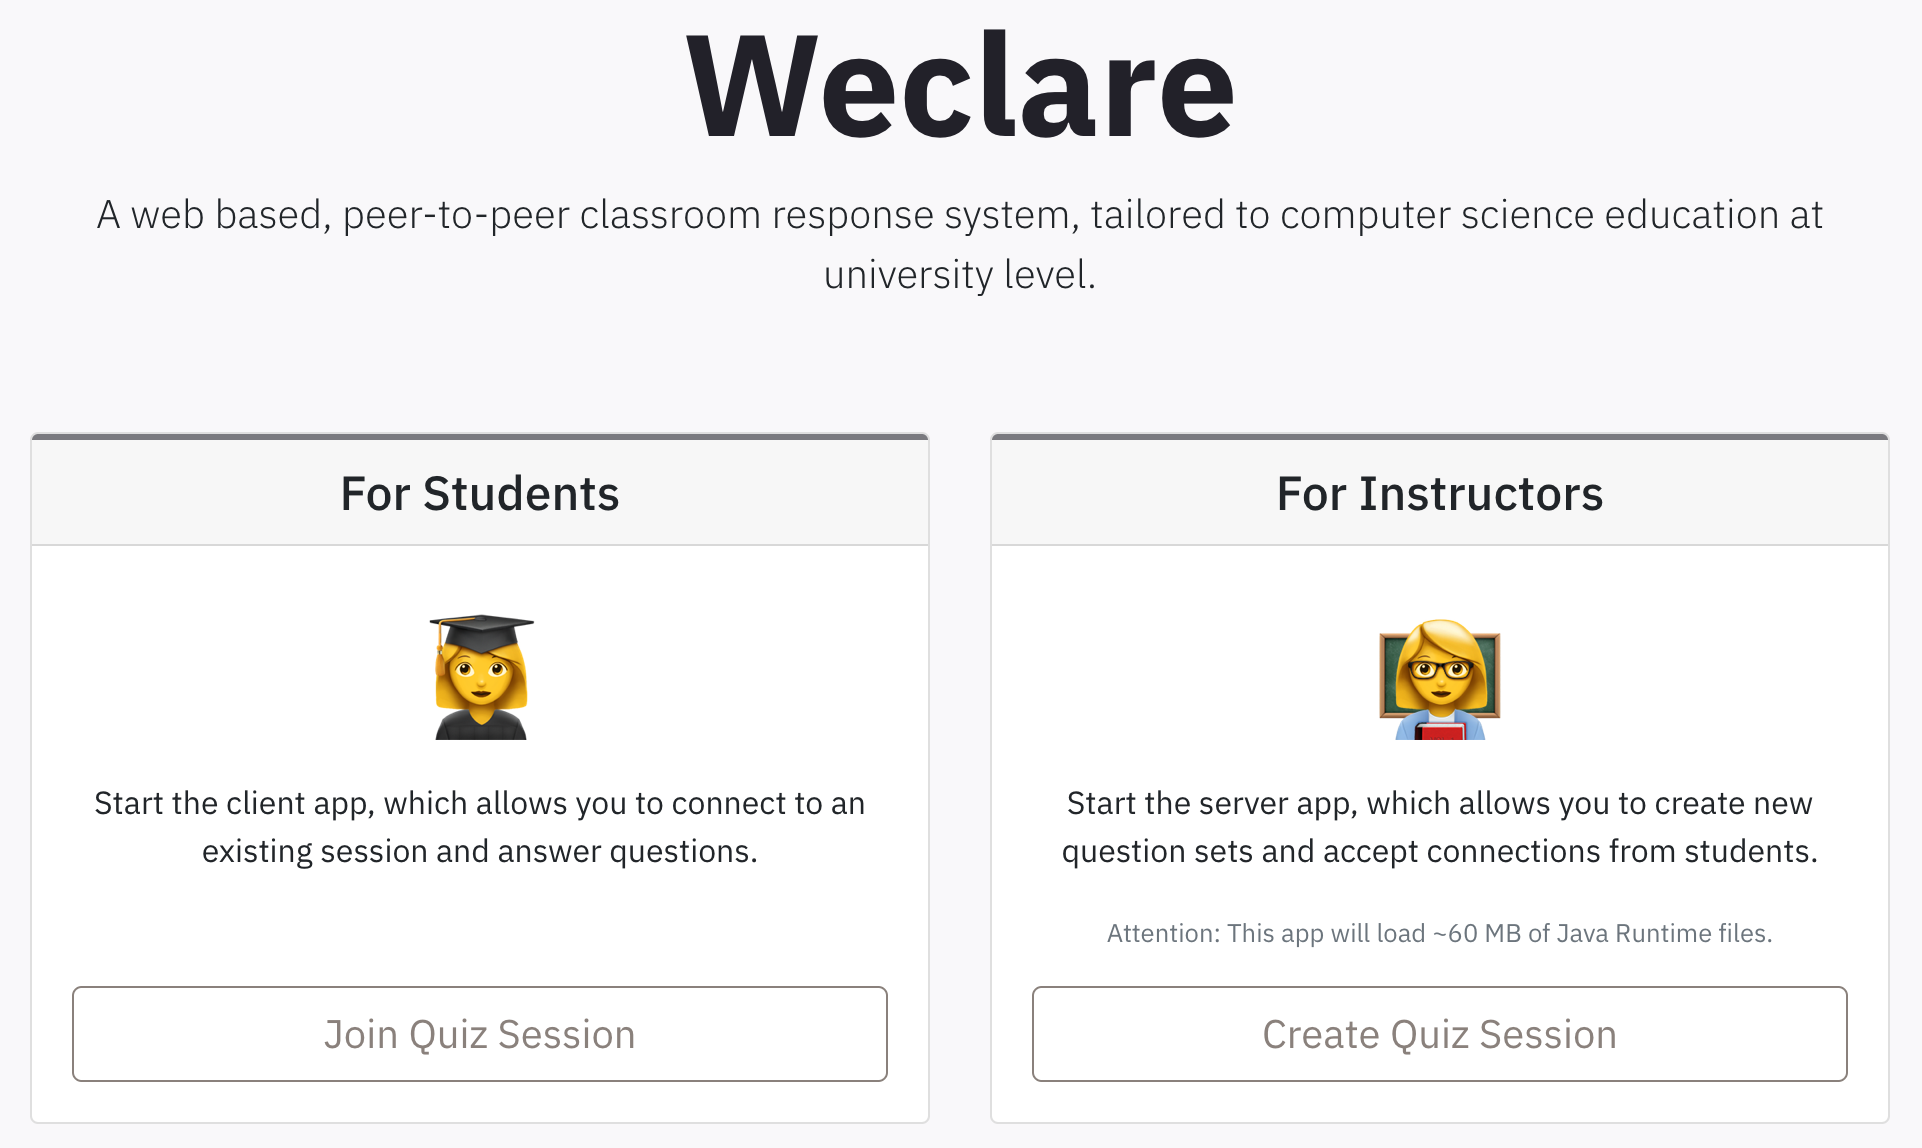
\includegraphics[width=\textwidth-1pt]{chapter/entwurf/bilder/weclare_start.png}}
    \caption[Start einer neuen Weclare-Sitzung]{Am Start einer Sitzung kann der Nutzer entscheiden, ob er als Client oder als Server teilnehmen möchte. Unabhängig von der Wahl wird das gleiche Programm geladen.}
    \label{abb:weclare_start}
\end{figure}

Mit diesem Verhalten erfüllt die Software die Definition einer Peer-to-Peer Architektur, zum Beispiel gemäß Tanenbaum\cite[S. 62]{book:tanenbaum}:

\begin{quotation}
„Aus einem übergeordneten Blickwinkel heraus sind die Prozesse, die ein Peer-to-Peer-System bilden, alle gleich. Die Funktionen, die ausgeführt werden müssen, werden also von jedem Prozess des verteilten Systems dargestellt. Folglich ist die meiste Interaktion zwischen Prozessen symmetrisch: Jeder Prozess agiert gleichzeitig als Client und als Server [...].“
\end{quotation}

Jedoch trifft dies eigentlich nur auf den Zeitraum vor dem Start einer Sitzung zu. Sobald eine Sitzung begonnen hat, handelt es sich um eine klassische Client-Server-Struktur. Die Bezeichnung als Peer-to-Peer-Architektur entspricht daher nicht der gängigen Vorstellung eines vollvermaschten Peer-to-Peer-Netzwerks, bei dem jeder Teilnehmer mit jedem anderen Teilnehmer verbunden ist.

Die Tatsache, dass jeder Teilnehmer entscheiden kann, ob er als Server oder Client teilnehmen will, bedeutet auch, dass Aspekte wie Network Address Translation (NAT) und Firewalls beim Austausch der IP-Adressen (Signaling) berücksichtigt werden müssen.

Der Zugriff auf die Schnittstellen des Betriebssystems (wie etwa das Netzwerk) durch Browser-Skripte ist aus Sicherheitsgründen stark eingeschränkt. Viele bestehende webbasierte CRS (zum Beispiel Pingo) verwenden das WebSocket-Protokoll zur Kommunikation zwischen Client und Server. Ein Browser kann jedoch nur ausgehende Verbindungen über WebSockets initiieren und nicht empfangen. Eine Peer-to-Peer-Architektur mit WebSockets ist deswegen nicht realisierbar.

Die einzige Möglichkeit, eine omnidirektionale Verbindung zwischen zwei Browsern zu realisieren, ist der relativ neue und offene WebRTC-Standard (Web Real-Time Communication)\footnote{Offizielle Webseite: \url{https://webrtc.org/}}. WebRTC wird hauptsächlich für Multimedia-Echtzeit-Anwendungen eingesetzt und seit 2017 von allen großen Browsern (Google Chrome, Mozilla Firefox, Opera, Apple Safari und Microsoft Edge) unterstützt. Viele Video- und Audiotelefonie-Lösungen (zum Beispiel Skype oder Discord) basieren inzwischen auf dem WebRTC-Protokoll. Neben Audio- und Videoinhalten können aber auch beliebige andere Daten über sogenannte \texttt{RTCDataChannel} übertragen werden. WebRTC beinhaltet aber keine Anweisungen für den Austausch der IP-Adressen zwischen beteiligten Parteien. Dieser Teil, das sogenannte Signaling, ist nicht Teil des Standards und muss selbst implementiert werden.

Der Aufwand dafür ist relativ groß, weil viele verschiedene Netzwerk-Situationen berücksichtigt werden müssen. Deswegen wird beim Weclare-Prototypen eine OpenSource-Bibliothek namens PeerJS\footnote{Offizielle Webseite: \url{https://peerjs.com/}} verwendet, die WebRTC in eine sehr einfache API kapselt und ein etabliertes Signaling-Verfahren beisteuert.

Die mehrfach formulierte Anforderung, keinen dedizierten Server zu benötigen, kann aufgrund des notwendigen Signalings also nicht vollständig erfüllt werden und muss an dieser Stelle präzisiert werden: Ein Server wird lediglich zum Austausch der IP-Adressen der Teilnehmer benötigt. Nach dem Austausch ist kein Server mehr notwendig. Anwendungsdaten werden nie über einen zentralen Server, sondern immer nur zwischen den einzelnen Teilnehmern verschickt (Die TURN-Funktionalität von WebRTC wird nicht verwendet). Der Signaling-Server muss nicht vom Weclare-Anwender betrieben werden – ein öffentlicher Server kann verwendet werden.

Die PeerJS-Library ermöglicht den Aufbau einer Datenverbindung zwischen zwei Browsern mit sehr simplen Aufrufen: Zunächst müssen Client und Server ein Peer-Objekt erzeugen. Als Parameter kann an dieser Stelle eine (auf dem Signaling-Server noch nicht verwendete) alphanumerische ID übergeben werden, unter welcher der zugehörige Peer beim Signaling-Server bekannt gemacht wird. Optional kann außerdem ein eigener Signaling-Server angegeben werden. Die Standard-Einstellung verwendet den kostenlosen und öffentlichen Signaling-Server, der von den PeerJS-Autoren betrieben wird.

Anschließend können an dem neuen Peer-Objekt diverse Callback-Methoden registriert werden, die den weiteren Gebrauch regeln. So kann zum Beispiel der Server seine neu erstellte ID kundtun und auf eingehende Verbindungen und Daten reagieren:

\begin{minipage}{\linewidth}
\begin{lstlisting}[caption={Verbindungsaufbau mit der PeerJS-Bibliothek auf der Server-Seite. (aus: src/server/actions/server.js)}]
import Peer from "peerjs";

const peer = new Peer("server-id");

peer.on("open", id => {
  console.log(`Successfully created peer: ${id}`);
});

peer.on("connection", conn => {
  console.log(`New client connected: ${conn.peer}`);
  conn.on("data", data => {
    switch (data.type) {
      case "answer":
        // Do something
        break;
      default:
      // Noop
    }
  });
});
\end{lstlisting}
\end{minipage}

Auf der Gegenseite, beim Client kann die Verbindung einfach über die \texttt{connect()}-Methode aufgebaut werden, die als Parameter die ID des gewünschten Peers erhält. Anschließend kann über das zurückgelieferte \texttt{Connection}-Objekt eine Nachricht verschickt werden:

\begin{minipage}{\linewidth}
\begin{lstlisting}[caption={Verbindungsaufbau mit der PeerJS-Bibliothek auf der Client-Seite. (aus: src/client/actions/client.js)}]
import Peer from "peerjs";

const peer = new Peer();
const connection = peer.connect("server-id");
connection.send("Hello world!");
\end{lstlisting}
\end{minipage}

Um dem Flux-Muster (siehe Kapitel \ref{chap:redux_state_management}) treu zu bleiben, wird die gesamte Netzwerk-Kommunikation innerhalb von ActionCreator-Funktionen implementiert. Da Netzwerk-Aufrufe keine puren Funktionen sind und asynchron erfolgen müssen, können sie nicht in einen reducer integriert werden. Um solche asynchronen Actions zu realisieren, wird Redux um eine sehr simple Middleware namens \texttt{redux-thunk}\footnote{Offizielle Webseite: \url{https://github.com/reduxjs/redux-thunk}} erweitert. Diese Middleware erlaubt es, asynchrone Aufrufe in ActionCreator-Methoden unterzubringen. Da viele dieser Netzwerkaufrufe eigentlich keine Änderungen im Store bewirken, wird der ActionCreator streng genommen missbraucht, denn am Ende wird, entgegen seinem Zweck, keine Action mehr zurückgegeben.

\begin{minipage}{\linewidth}
\begin{lstlisting}[caption={ActionCreator zum Versenden von Antworten vom Client zum Server. (aus: src/client/actions/client.js)}]
export function sendAnswers(answerIdxArray) {
  return (dispatch, getState) => {
    const {
      client: { connection = null, currentQuestion = null }
    } = getState();

    if (
      connection &&
      currentQuestion &&
      typeof answerIdxArray !== "undefined"
    ) {
      const msg = {
        type: "answer",
        payload: {
          questionIdx: currentQuestion.questionIdx,
          answerIdxArray,
          userId: connection.provider.id
        }
      };
      connection.send(msg);
    }
  };
}
\end{lstlisting}
\end{minipage}